\documentclass[10pt,twocolumn, nofootinbib]{revtex4-1}
%\documentclass[aps,pra,10pt,twocolumn,floatfix,nofootinbib]{revtex4-1}
%\documentclass[10pt,twocolumn,letterpaper]{article}

\usepackage{amsmath}
\usepackage{amsfonts}
\usepackage{amsthm}
\usepackage{MnSymbol}
\usepackage{graphicx}
\usepackage{enumitem}
\usepackage{hyperref}
\hypersetup{
	colorlinks=true,
	citecolor=blue,
	urlcolor=blue,
	linkcolor=blue
}
\urlstyle{same}
\frenchspacing

\newtheorem{prop}[equation]{Proposition}

\begin{document}

\title{Notes on classical/quantum logic }
\author{Gabriele Carcassi, Christine A. Aidala}
\affiliation{Physics Department, University of Michigan, Ann Arbor, MI 48109}

\date{\today}


\begin{abstract}
Notes of classical logic in quantum mechanics.
\end{abstract}

\maketitle

\section{Quantum logic: definition and motivation}

\subsection{Disjunction}

Connection between disjunction and superposition.

``A relevant feature of $\vee$ is that, differently from the case in classical semantics, a quantum disjunction may be true even if neither of it members is true. This reflects, for example, the case in which we are dealing with a state such as that of a spin 1/2 system which is in a linear combination of states up and down. Both propositions, ``the state is up'' and ``the state is down,'' may have no definite truth value (the excluded middle principle is violated), but the disjunction ``the state is up or the state is down'' is a tautology.''

\begin{description}
	\item $p =$ ``The particle has spin $z^+$''
	\item $q =$ ``The particle has spin $z^-$''
\end{description}

Claim: $p \vee q$ is \textbf{always} true, even if $p$ and $q$ may possibly be both false. The idea is that $p \vee q$ includes also all superpositions of $p$ and $q$.

Counterclaim. The propositions $p$ and $q$ are experimentally equivalent to:
\begin{description}
	\item $p =$ ``The expectation value for $S_z$ is 1/2$\hbar$''
	\item $q =$ ``The expectation value for $S_z$ is -1/2$\hbar$''
\end{description}
The proposition $p \vee q$ corresponds to the statement ``The absolute value of the expectation value for $S_z$ 1/2$\hbar$''. If we have a superposition of $p$ and $q$, the expectation value for $S_z$ will be strictly between $-1/2 \hbar$ and $1/2 \hbar$, and therefore $p \vee q$, when discussing expectation values, will be false as one would expect.

\subsection{Distributivity}

The distributivity in quantum mechanics is ``weird'' because (1) it can be true even if none of the elements of the disjunction is true due to the linearity of the Schroendinger equation and (2) quantum observables do not commute. 

\begin{description}
    \item $p =$ ``The particle has spin $x^+$''
    \item $q =$ ``The particle has spin $y^+$''
    \item $r =$ ``The particle has spin $y^-$''
\end{description}

Classic: $p \wedge (q \vee r)$ if and only if $(p \wedge  q) \vee (p \wedge r)$

Quantum: Assume $p$ is true, which means we measured spin $x$ to be $+$. Since if I measured spin $y$ I would either get $+$ or $-$, we have $q \vee r \equiv \top$. Therefore $q \vee r \equiv \top$ is true. On the other hand, both terms in the second disjunctions are false: because $p \wedge  q$ refer to incompatible observables, we have $p \wedge  q \equiv \bot$. Therefore the $(p \wedge  q) \vee (p \wedge r) \equiv \bot$.

$q \vee r \equiv \top$ therefore $p \wedge (q \vee r) \equiv p \wedge \top \equiv p$. If $p$ is true

\subsubsection{Reframing}

\begin{description}
    \item $p =$ ``The state of particle at time $t$ is $x^+$''
    \item $q =$ ``The state of particle at time $t$ is $y^+$''
    \item $r =$ ``The state of particle at time $t$ is $y^-$''
\end{description}

Then all three assertions are incompatible with each other. That is, $p \wedge q \equiv q \wedge r \equiv r \wedge p \equiv \bot$. Therefore $p \wedge (q \vee r) \equiv \bot \equiv (p \wedge  q) \vee (p \wedge r)$.

2 casi: considerare

\begin{description}
    \item $p =$ ``The state of particle at time $t$ is $x^+$''
    \item $q =$ ``The state of particle at time $t$ is $y^+$''
    \item $r =$ ``The state of particle at time $t$ is $y^-$''
    \item $\hat{q} =$ ``The state of particle at time $\hat{t}$ is $y^+$''
    \item $\hat{r} =$ ``The state of particle at time $\hat{t}$ is $y^-$''
\end{description}

In this case $p \wedge \hat{q} \nequiv \bot$ and $p \wedge \hat{r} \nequiv \bot$. Therefore the original claim was $p \wedge (\hat{q} \vee \hat{r})$ if and only if $(p \wedge  q) \vee (p \wedge r)$ which is not the classical logic distributive law. Note that, $\hat{q} \vee \hat{r} \equiv \top$ under condition that ``We measure spin $y$ at time $\hat{t}$''.

\subsubsection{Classical example}
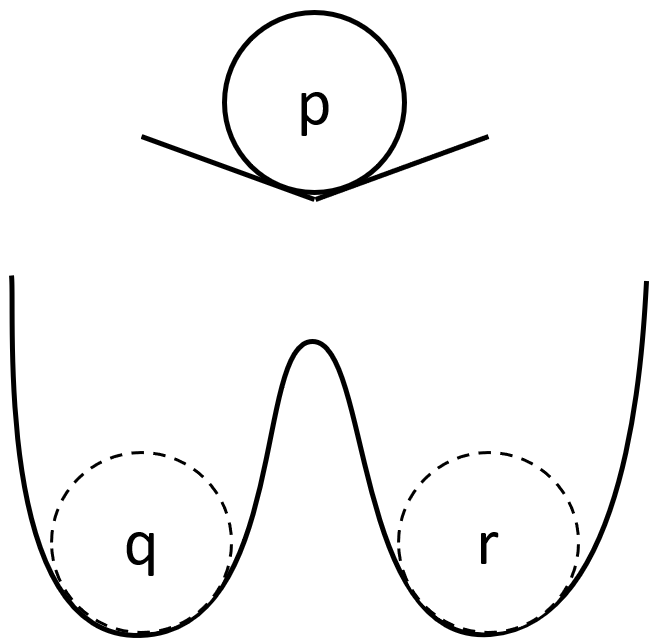
\includegraphics[width=\columnwidth]{Balldrop.png}

We have a ball sitting at position $p$ over a hatch. If the hatch opens, the ball drops, bounces around, until it will rest at either position $q$ or $r$ with equal chance. Two cases, as before:

\begin{description}
    \item $p =$ ``The position of the ball at time $t$ is $p$''
    \item $q =$ ``The position of the ball at time $t$ is $q$''
    \item $r =$ ``The position of the ball at time $t$ is $r$''
\end{description}

These are three incompatible assertions. Distributivity holds as before.

\begin{description}
    \item $p =$ ``The position of the ball at time $t$ is $p$''
    \item $q =$ ``The position of the ball at time $t$ is $q$''
    \item $r =$ ``The position of the ball at time $t$ is $r$''
    \item $\hat{q} =$ ``The position of the ball at time $\hat{t}$ is $q$''
    \item $\hat{r} =$ ``The position of the ball at time $\hat{t}$ is $r$''
\end{description}

We assume that, after time $t$, the hatch is opened and that at time $\hat{t}$ the ball has settled. As before, $\hat{q} \vee \hat{r} \equiv \top$ because the ball must be in one of the two positions after it dropped, therefore, if $p$ is true, the left side of the biconditional is true while the right side is false.

\section{Classical and quantum parallel}

Classical state: $\rho(x,p)$

Quantum state: $\psi(x)$

Classical observable $f(x,p)$. Average value $<f> = \int f(x, p) \rho(x, p) dx dp$. Eigenstate $f(x, p) \rho(x, p) = f_0 \rho(x, p)$.

Quantum observable $F$. Average value $<F> = \int \psi^\dagger(x) F \psi(x) dx$. Eigenstate $F \psi(x) = f_0 \psi(x)$.

In both cases, average value equal to $f_0$ means that the contributions of all parts of the ensemble combine to the value $f_0$. Eigenstate $f_0$ means all parts of the ensemble contribute the same value $f_0$.

For example, a classical eigenstate of $H = \frac{p^2}{2m} + \frac{1}{2} k x^2$ with eigenvalue $e_0$ is any function $\rho(x,p)$ that is different from zero only on the ellipses with energy $e_0$. That is, all elements of the distribution have the same energy.

The statement ``the observable $f$ of the system is between $f_0$ and $f_1$'' is therefore unclear. It could be taken to mean ``the average of observable $f$ of the system is between $f_0$ and $f_1$'' or ``the observable $f$ for each part of the ensemble is between $f_0$ and $f_1$''. In the first case, we are identifying a value from the real line, using the standard topology and the standard Borel algebra. In the second case, we are identifying a set of possible functions based on their support.

Now suppose that the $U$ and $V$ are two intervals. We have ``the average $<f>$ is in $U \cup V$'' is  equivalent to ``the average $<f>$ is in $U$'' $\vee$ ``the average $<f>$ is in $V$''. The average value must be in and and only one set. We also have ``the support of $\rho$ is $U \cup V$'' is not equivalent to ``the support of $\rho$ is $U$'' $\vee$ ``the support of $\rho$ is $V$''. The dis tribution could span both sets at the same time. But the lattice generated by such sets is still a $\sigma$-algebra, and therefore follows classical logic.

To check/prove: neither algebras is a sub-algebra of the other; both sub-algebras of the norm-induced one.

\section{Math}

In this section, we want to show how Hilbert spaces already are equipped with a mathematical structure that follows classical logic, namely the Borel algebra. We will see that the algebra typically associated with quantum logic is a subset of this structure. We will see that this classical structure contains other statements that are experimentally significant, like statements about the expectation values. Finally, we will show that the algebra of subspaces of classical distributions is also non-distributive in the same way that quantum logic is.

Let us start with a brief summary of the basic mathematical structure of quantum logic. Each proposition for a Hilbert space $H$ correspond to a closed subset. This forms a complete lattice under the following definitions: the ordering $p \leq q$ of the lattice (i.e. the implication $p \to q$) represents subspace inclusion, the conjunction $p \wedge q$ is the biggest subspaces contained by both, the disjunction $p \vee q$ is the smallest subspace that contains both, the negation $\neg p$ is the orthogonal subspace.

To understand how the previous structure fails to a be Boolean algebra, we note that by Stone's representation theorem any Boolean algebra can be expressed as an algebra of sets using the standard set operations (i.e. inclusion, intersection, union and complement). If we understand each subspace as a set of vectors, the conjunction $p \vee q$ is not the mere set union of the subspaces, but the span. This is why the above structure, even if it is a complemented $0-1$ lattice, it fails to be a Boolean alebgra.

However, a Hilbert space $H$ is a complete normed space. The norm induces a topology, which in turns induces a Borel-algebra. The Borel-algebra is a family of sets closed under countable intersection, union and negation. It therefore forms a Boolean algebra. Therefore propositions of the type ``the state is in set $A$'' for any Borel set $A$ follow the rules of classical logic.

Note that the lattice of quantum logic is formed by closed subspaces, which are closed sets and therefore Borel sets. Therefore all statements expressible in quantum logic (e.g. ``we measured/prepared this quantity with the following value'') are also expressible with the Borel algebra. The converse, however, is not true: not all Borel sets correspond to propositions in quantum logic.

To show that some of these statements are indeed interesting, let us consider the following result:
\begin{prop}
	Let $H$ be an Hilbert space and $\langle \, , \, \rangle$ be its inner product. Let $X$ be a self-adjoint bounded linear operator. Let $F_X : H \to \mathbb{R}$ the map defined by $F_X(\psi) = \langle \psi , X \psi \rangle$. Let $U \subseteq \mathbb{R}$ be a Borel set. Then $F_X^{-1}(U)$ is a Borel set.
\end{prop}

A proof would work along these lines. A linear operator between two normed spaces is continuous if and only if it is bounded, therefore our operator $X$ is continuous. Since the inner product is also continuous, $F_X$ is continuous. Since $F_X$ is continuous, the reverse image of an open set is an open set. Since a Borel set $U$ can be constructed from open sets using negation and countable union, the reverse image $F_X^{-1}(U)$ can also be constructed from open sets using negation and countable union, which means it is a Borel set.

Since $\langle \psi , X \psi \rangle$ expresses the expected value for operator $X$, the proposition shows that the Borel algebra can express statements about the expectation value of observables,\footnote{Technically, position and momentum are not bounded operators. However, one can argue that measured position and momentum are indeed bounded as the acceptance of a detector is always limit. Note that all operators for which the spectral theorem applies can be written as the limit of a sequence of bounded operators.} such as ``the expected position $\langle x \rangle$ of the particle is between $x_0$ and $x_1$.'' This would correspond to the Borel set $\{ \psi \in H \, | \, \langle \psi , X \psi \rangle \in (x_0, x_1) \}$.\footnote{In most cases, one assumes states to be normalized, which is what we have done here for simplicity. Renormalization would lead to the set $\{ \psi \in H \, | \, \langle \psi , X \psi \rangle / \langle \psi , \psi \rangle \in (x_0, x_1) \}$, which is still a Borel set since renormalization is a continuous function over its domain $H \setminus \{ 0 \}$.}

Borel sets allow us to express statements such as ``the expected position $\langle x \rangle$ of the particle is exactly $x_0$''. This is NOT equivalent to the statement ``the particle is in the eigenstate $x_0$''. The second will be true only if the whole function is at $x_0$. That is, if the $x_0$ is the support of the wave-function. The first is a lot less stringent: the wave-function can even be distributed over an infinite range (e.g. a Gaussian wave packet) just as long the average is $x_0$. This means that we can have statements like ``the expected position $\langle x \rangle$ of the particle is exactly $x_0$''$\wedge$ ``the expected momentum $\langle p \rangle$ of the particle is exactly $p_0$'' without having contradictions (e.g. a Gaussian wave packet can be centered any value of position and momentum).

Note that all statements that characterize the position and momentum of the center mass and form a sub-algebra of the Borel algebra. If the potential for a quantum particle can be considered constant over the wave-function (i.e. $\langle V(x) \rangle = V(\langle x \rangle)$ ), the motion of the center of mass will reduce to the case of a point-particle. In fact, this is exactly how the point particle approximation arises in classical mechanics as well: when we study the motion of planets, cannonballs or specs of dust, we understand that these objects are not point-like, but they have an extent and a matter distribution. The point-particle approximation works insofar we are interested in the motion of the center of mass and the forces are such that the extent of the object does not matter. Naturally, if the orbit of a planet would be such that its distance is less than the radius of the sun, the point-particle approximation would fail spectacularly. In this regard, quantum mechanics works the same way.

Now that we have shown that quantum mechanics can be given an algebra that looks more like the one of classical mechanics, let us do the converse: show that we can (at least formally) give classical mechanics an algebra that looks like the one of quantum logic. As we said before, classical objects are not point-like. So let us consider the space of all possible matter distributions $\rho(x,p)$ over phase-space. We can formalize this as a Hilbert space, where vector $\psi$ corresponds to $\sqrt{\rho(x,p)}$. This will be a real vector space, and we are only going to consider operators that can be expressed as a multiplicative function $f(x,p)$. Note that $\langle \psi | F \psi \rangle = \int f(x,p) \rho(x,p) dx dp$ as one would expect.\footnote{To be clear: we are not arguing that this construction is the most appropriate or useful. Simply that it can be done.}  We can now take the algebra of subspaces and, as in the quantum case, it will be non-distributive: the disjunction of two subspaces will not be the set union, but the span.

To simplify, let us assume that there are only two possible states $1$ and $2$. A state is identified by a two-valued distribution $[\rho_1, \rho_2]$, which we can take it to be either the probability of the particle being in each state or the amount of material in each state. We note $[k,0]$ the subspace spanned by the first state only. This corresponds to the case where the whole system is in state $1$. Conversely, $[0,k]$ corresponds to the case where the whole system is in state $2$. The disjunction $[k,0] \vee [0,k]$ will correspond to the state spanned by both, which is the whole space $[k,j]$. We can also take the subspace $[k,k]$ which is the subspace spanned by vectors that have equal components in $1$ and $2$: the system is equally distributed in the two cases. Note that $[k,0]$, $[0,k]$ and $[k,k]$ are all pairwise disjoint: no pair have a vector in common apart from zero. Therefore their conjunctions $[k,0] \wedge [0,k] = [0,k] \wedge [k,k] = [k,k] \wedge [k,0] = [0,0]$ are the zero dimensional. On the other hand, $[k,k]$ is a subspace of the whole space $[k,j]$ and therefore $[k,k] \wedge [k,j] = [k,k]$. Putting it all together, we have $[k,k] \wedge ( [k,0] \vee [0,k] ) = [k,k] \wedge [k,j] = [k,k]$. On the other hand, $( [k,k] \wedge [k,0] ) \vee ( [k,k] \wedge [0,k] ) = [0,0] \vee [0,0] = [0,0]$. Therefore the lattice is not distributive.

The lack of distributivity has nothing to do with the complexity of the Hilbert space or non-commuting observables. It's a property of the lattice of subspaces of a vector spaces. In fact, it's a property of the lattice on subgroups more in general. In the subgroup lattice, the disjunction is the span, so doing the disjuction first makes our set bigger during the calculation. Naturally, one may still argue that it is appropriate to focus on this lattice in quantum mechanics while it is not appropriate for classical mechanics. But one cannot argue that this difference is a fundamental difference in the mathematical or logical structure of theories. Certainly, one cannot say that quantum mechanics requires a departure from classical mechanics when both theories follow similar structures.

The key difference between the algebras of statements, then, is not really about the type of the logical structure: it is its content in terms of statements. If we take two intervals $U_x$ and $U_p$ in position and momentum, and form the statement ``the state is wholly in $U_x$ and $U_p$'', meaning that the vector components are zero outside of those regions, in the classical case we always find at least one $\rho(x,p)$ that satisfies the bounds, while in quantum mechanics, if the bounds violate the uncertainty principle, no suitable $\psi(x)$ can be found. It is the content of the logic that changes. 

\section{Old notes}

* We can always use the Borel algebra for our statements. This will include(?) all propositions of ``quantum logic''.

It includes (?) also proposition on expectation values, say of position and momentum. Those will behave exactly like ``point particles''. It also includes (?) propositions on the support.

Show that this is similar to classical distributions.


Claim: in quantum mechanics the ``correct'' logical structure the is algebra of subspaces of the Hilbert space. In this algebra (which is a $\cap$-structure) the meet functions differently than in Boolean logic. Therefore it does not follow classical logic.

Resolution: that algebra does not include many statements that are interesting experimentally. For example, it does not include statements about the expectation values which, in the end, are the result of experiments. (Cross-section?) One 


Technical view: the state space of quantum states is a separable Hilbert space; it is a Banach space (complete normed space) and admits a norm-induced topology; it is separable, so it admits a countable basis, so the topology is second countable; therefore the state space has a countably generated Borel-algebra. This, like any set theoretic structure, follows Boolean algebra. Each state is a point and state-statements like ``the system is in state $s_1$'' are singletons in the $\sigma$-algebra. State-statements are all incompatible with each other: either we prepared one state or we prepared another.

If a process with an initial and final state (the internal are disregarded), we have two lattices of propositions. The sample space is the Cartesian product, the $\sigma$-algebra is the product. A measurement process will follow this pattern. We can say ``the system was prepared in state $s$'' and ``the system was measure in state $s$'' and there are two different statements. In the product algebra, we can then mix and match statements with the usual Boolean constructs. Both these are analogous in a classical and quantum case. These will naturally result in different lattices, but they will still be Boolean lattices.

What changes are the probability spaces we can construct. In the quantum case, the probability is not in general a probability measure and has to be consistent with the Born rule (i.e. the inner product).


\bibliography{quantumlogic}


\end{document}
